\section{Stair Detection}

% Description
In real-world application, the staircase is a common terrain occurrence. The robot is expected to navigate this terrain autonomously and with ease, thus requiring the implementation of stair detection. The stair detection algorithm takes images of stairs as primary input from the stereo camera setup. With the help of OpenCV fused with Hough Lines algorithm, the raw image data is further processed and refined to produce information about the stair contours, number of steps and step height.\\

% Flowchart
\begin{figure}[H]
    \centering
    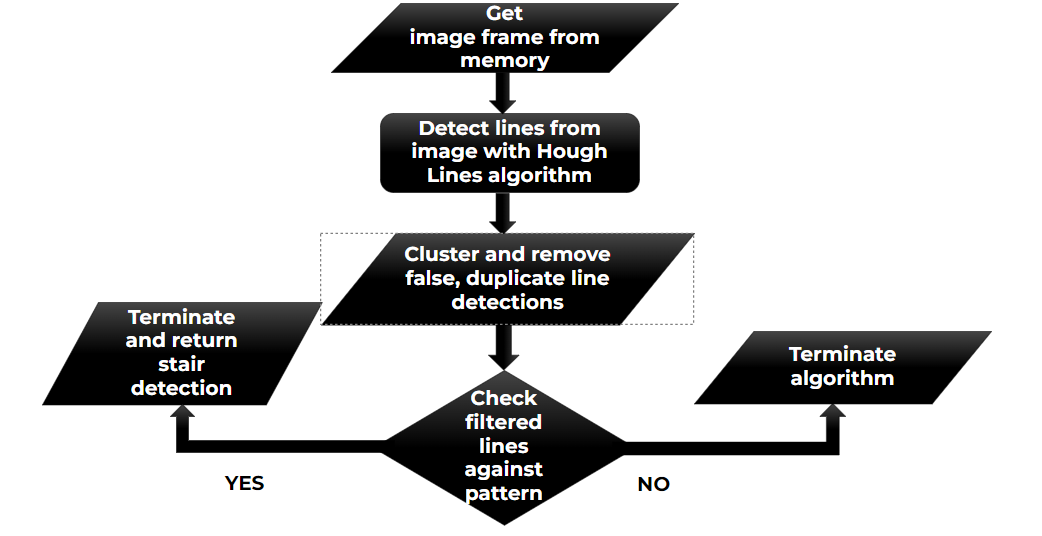
\includegraphics[width=0.9\textwidth]{stairDetect}
    \caption{Flowchart}
    \label{fig:stairDetectionFlowchart}
\end{figure}

% Algorithm
\begin{algorithm}[hbt!]
    \caption{Stair detection algorithm}\label{alg:cap}
    
    \begin{algorithmic}[1]
    
        \Require $img \gets Image\ data\ from\ stereo\ camera$
        \State $Binarize\ img\ to\ reduce\ noise$
        \State $Apply\ Canny\ Edge\ filter\ to\ img$
        \State $Apply\ Hough\ Lines\ filtering\ algorithm\ to\ img$
        \If {$0.1 < \theta < 0.8$}
            \State $\theta =Stair\ side\ angle:Left$
            \State $angleL \gets \theta$
        \ElsIf {$2.4 < \theta < 3$}
            \State $\theta = Stair\ side\ angle:Right$
            \State $angleR \gets \theta$
        \EndIf
        \State $Print\ angleL,\ angleR$
        \If {$91\times \frac{\pi}{180} < \theta <90 \times \frac{\pi}{180}$}
            \State $\theta =Stair\ angle: Vertical $
            \State $angleV \gets \theta$
        \EndIf
        \State $Overlay\ lines\ on\ img$
        \\
        \Return $img$
        
    \end{algorithmic}
\end{algorithm}

\newpage

\begin{figure}[H]
  \centering
    \begin{multicols}{2}
        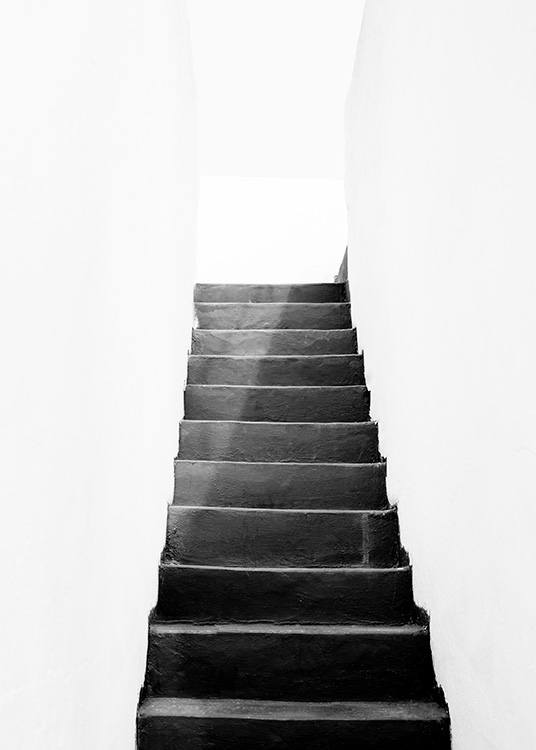
\includegraphics[width=0.4\textwidth]{stairDetectTest_1}
        \caption{Test image}
        \label{fig:testImage}
        
        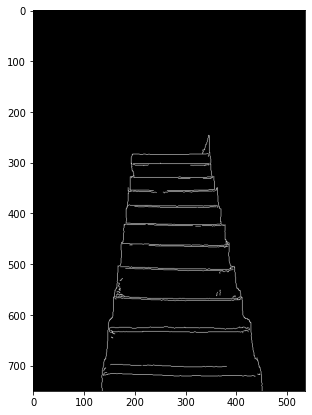
\includegraphics[width=0.45\textwidth]{stairDetectTest_2}
        \caption{Processed image}
        \label{fig:processedImage}
    \end{multicols}     
\end{figure}

\begin{figure}[H]
  \centering
    \begin{multicols}{2}
        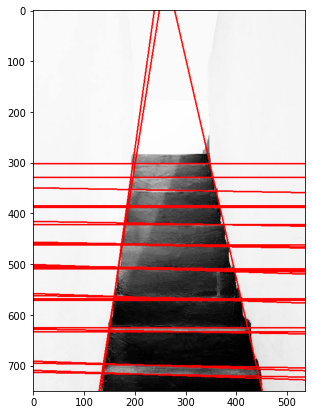
\includegraphics[width=0.4\textwidth]{stairDetectTest_3}
        \caption{Applying Hough Lines algorithm}
        \label{fig:horizontalLinesRaw}
        
        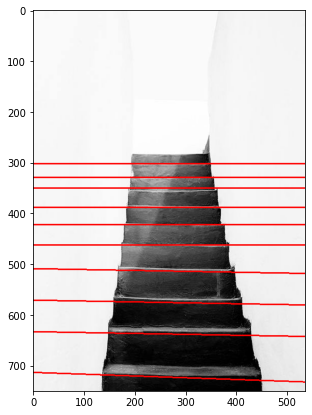
\includegraphics[width=0.4\textwidth]{stairDetectTest_4}
        \caption{Flitered final image}
        \label{fig:horizontalLinesFiltered}
    \end{multicols}     
\end{figure}